\section{Design}
Broadly speaking, the design of what will be added and changed to the newly revised CloudSentinel framework can be put in four categories, starting with the 'Data Catalogue' component. This chapter covers each of these categories.

\subsection{Data Catalogue}
The evaluation concluded that data gathering in particular is one difficult part of CloudSentinel, as was also pointed out in the CloudSentinel evaluation of Van Gaalen (2024). CloudSentinel does not offer any mechanism that operators can use to gather a metrics dataset for the model-training. As a consequence, operators are forced to use their own roudabout mechanisms, such as custom scripts, to pull prometheus data  themselves, as well as put them in the right feature-column format and scale their values accordingly, such that they can be interpreted correctly by the anomaly detection algorithm in training. Furthermore, there is no data provenance present; meaning that once a model has been trained, the dataset that was used is not recorded and cannot be analysed at a later point.\\

In order to address these issues, we introduce a 'data catalogue' component. The data catalogue lets operators define and store dataset configurations as persistent objects, fetch the corresponding datawindows from Prometheus, and reuse these as many times as desired in different parts of the applications. It is intended to transform dataset management from tedious manual work into a task completed with a few button clicks.\\

In addition to descriptive metadata such as a dataset name and description, operators can assign a 'context workload' to each dataset. This categorises the dataset according to relevant workload characteristics, such as high or low CPU load. Although this information is not strictly required for model training, it is useful in that it helps operators distinguish between datasets and assess which types of workloads detector models identify effectively- and where their performance is limited.\\

The following figures give a low-fi overview of the user interface of the data catalogue component. Figure \ref{fig:data_cat_overview} displays the overview screen where users are able to view an overview of all the saved datasets. Figure \ref{fig:data_cat_add_dataset}  shows the 'add dataset' screen where users can define a new dataset. Figure \ref{fig:data_cat_view_dataset} displays the 'view dataset' screen, where users can view a saved dataset in detail.

\begin{figure}[H]
    \centering
    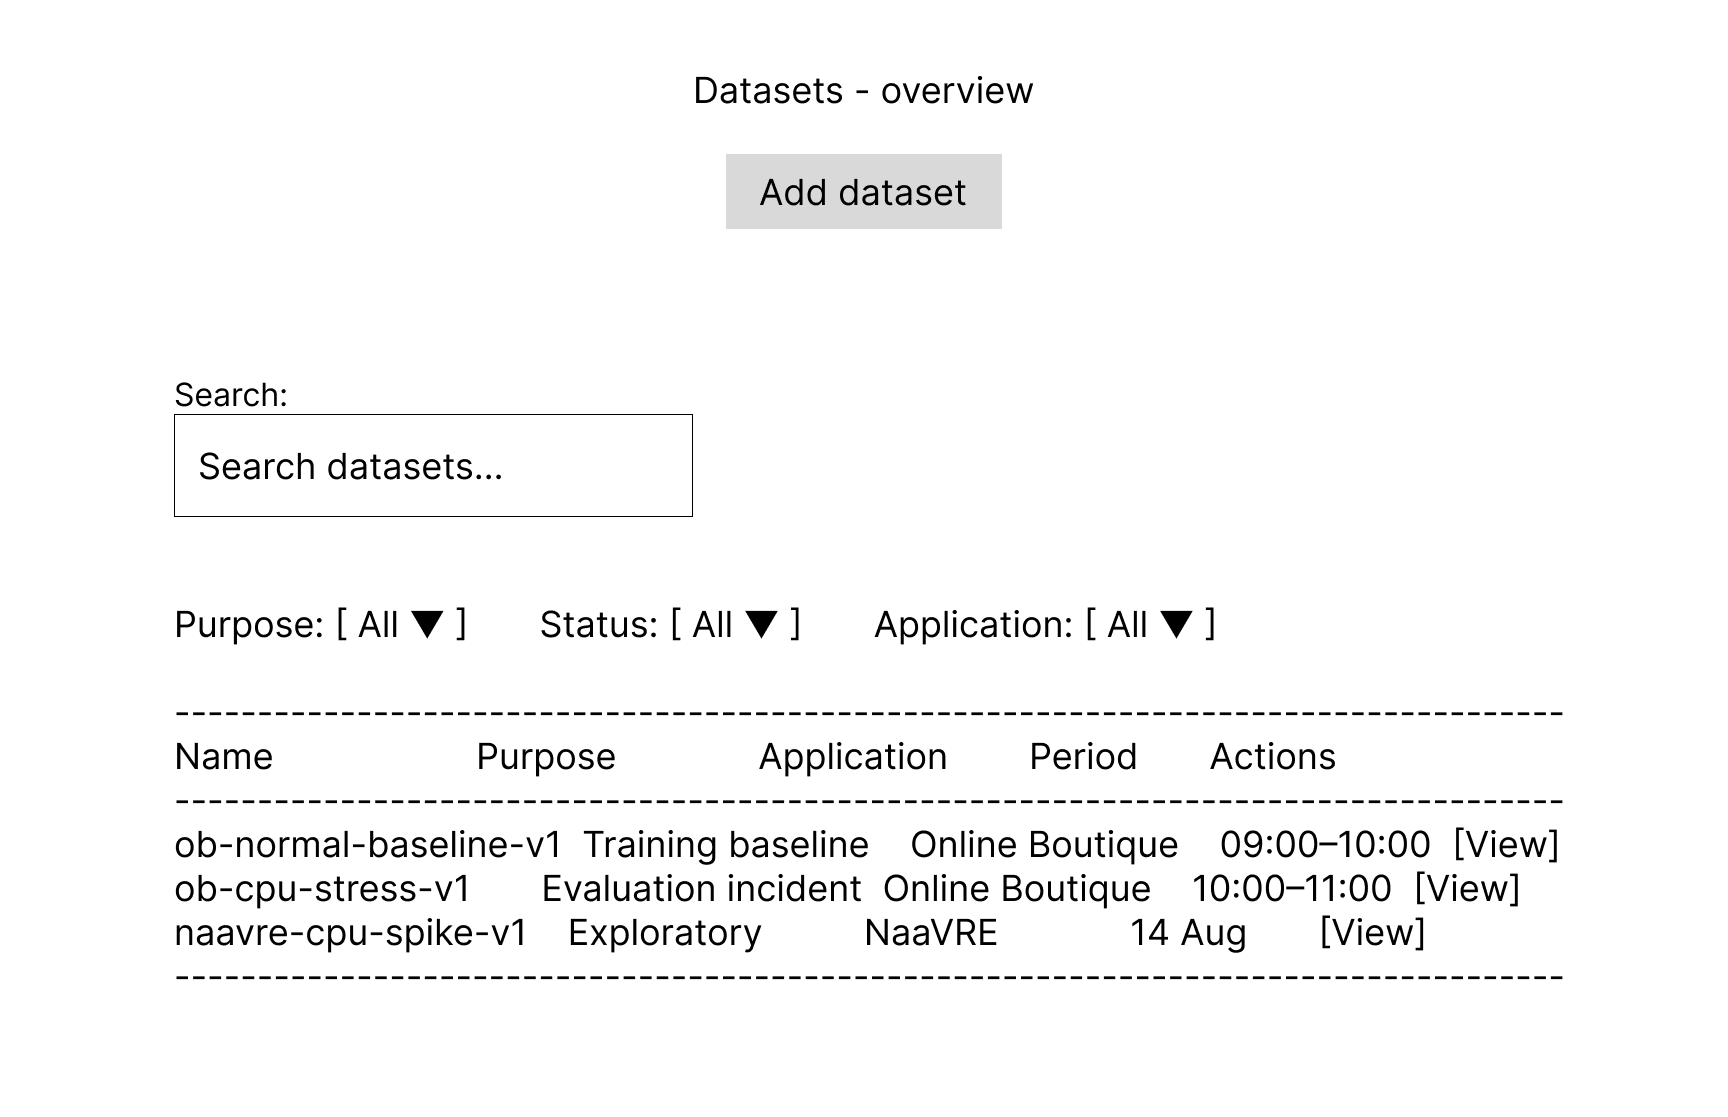
\includegraphics[width=1\linewidth]{figures/design/data_catalogue/Data Catalogue - overview.png}
    \caption{Data Catalogue: Overview}
    \label{fig:data_cat_overview}
\end{figure}

\begin{figure}[H]
    \centering
    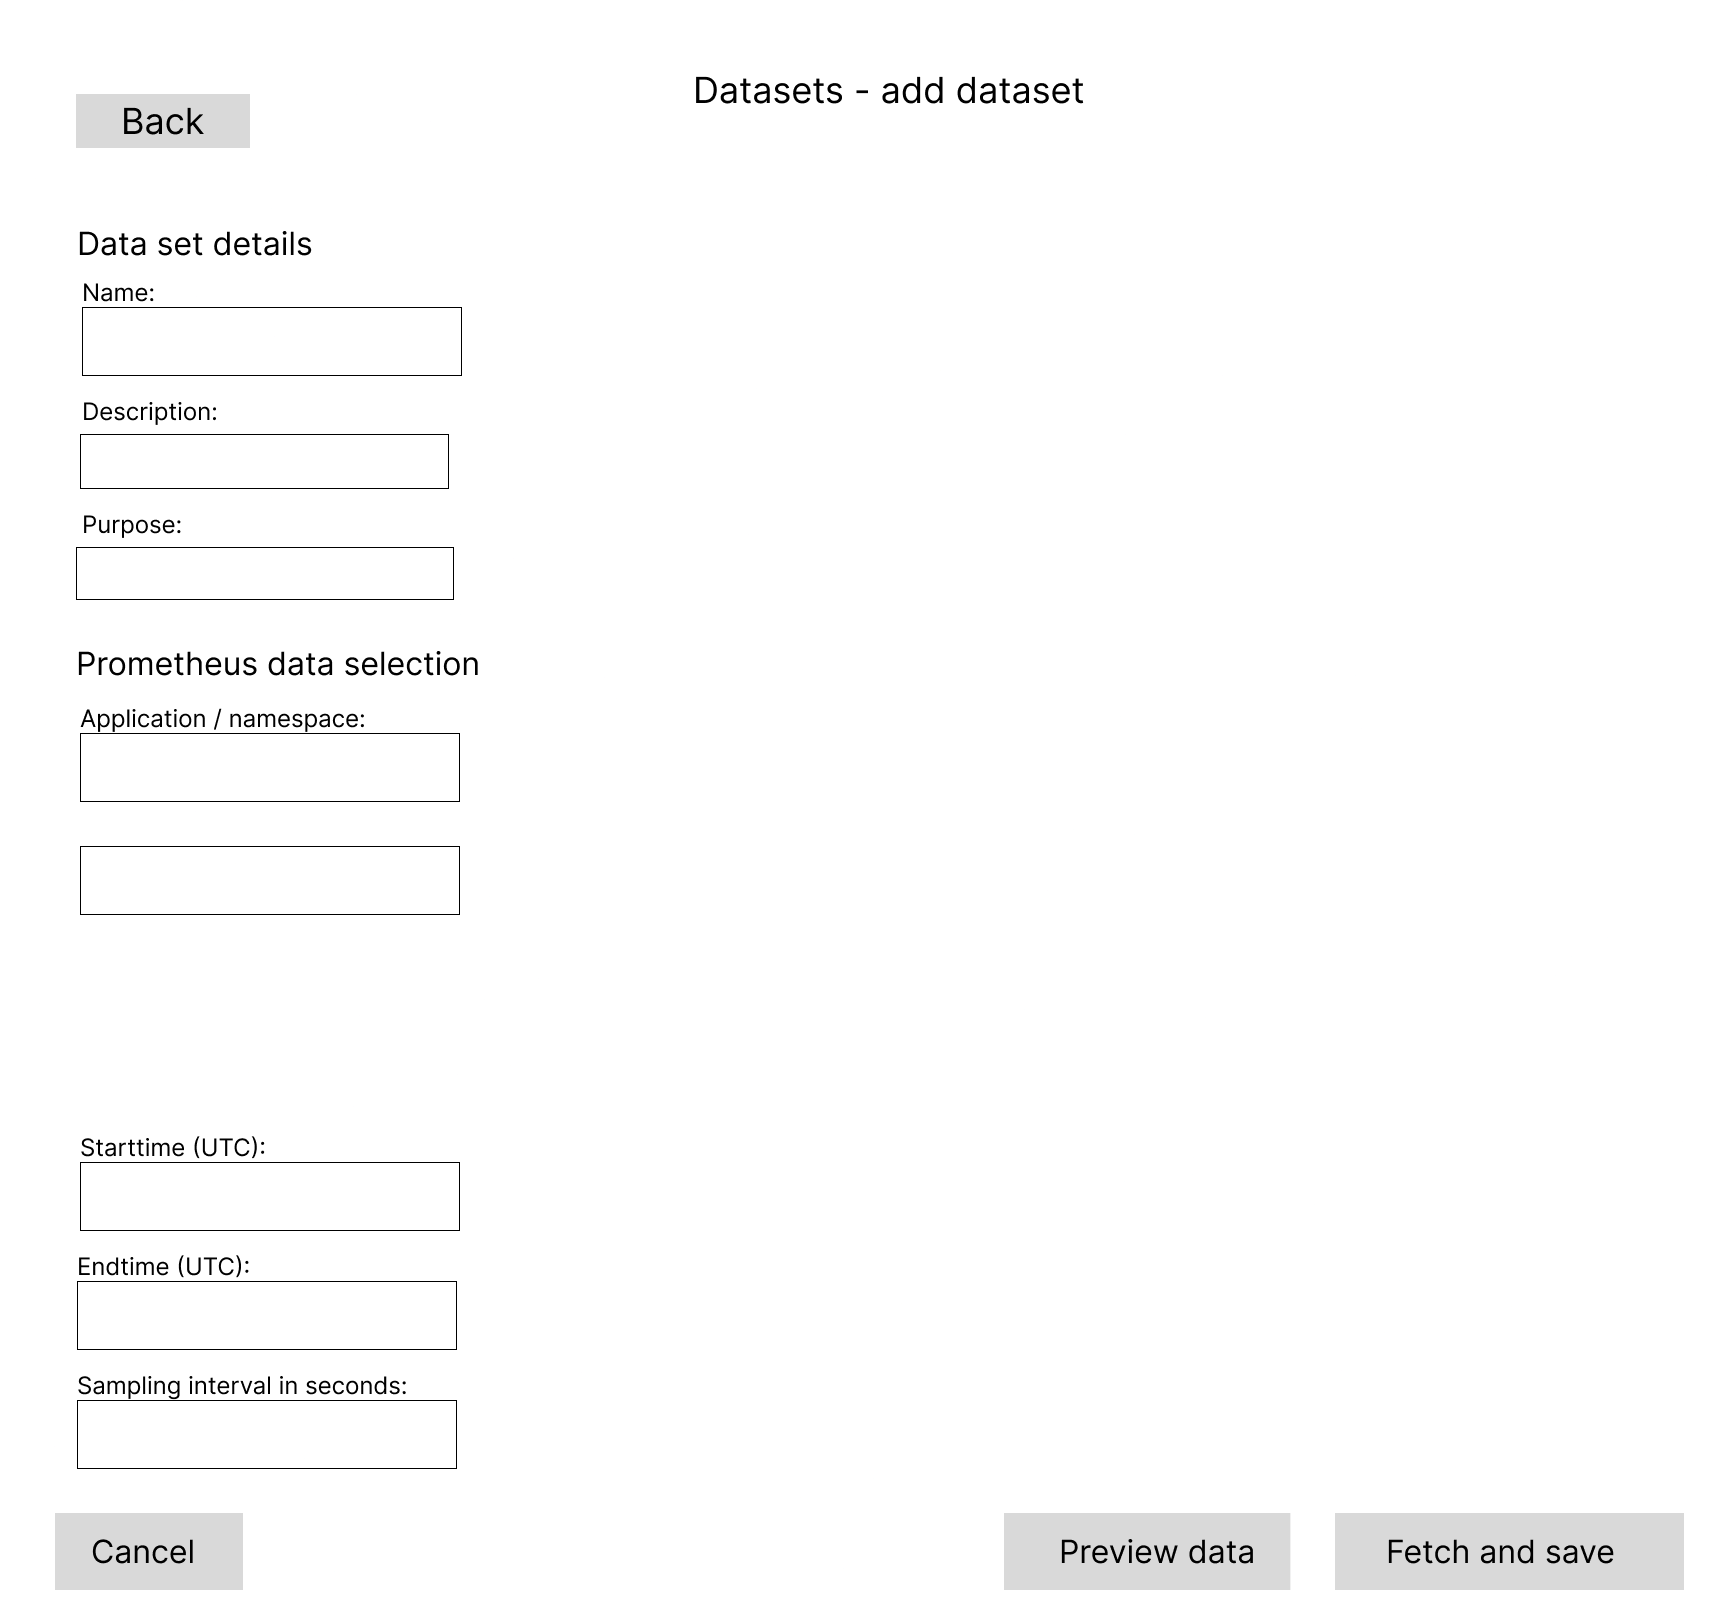
\includegraphics[width=1\linewidth]{figures/design/data_catalogue/Data Catalogue - add dataset.png}
    \caption{Data Catalogue: Add dataset}
    \label{fig:data_cat_add_dataset}
\end{figure}

\begin{figure}[H]
    \centering
    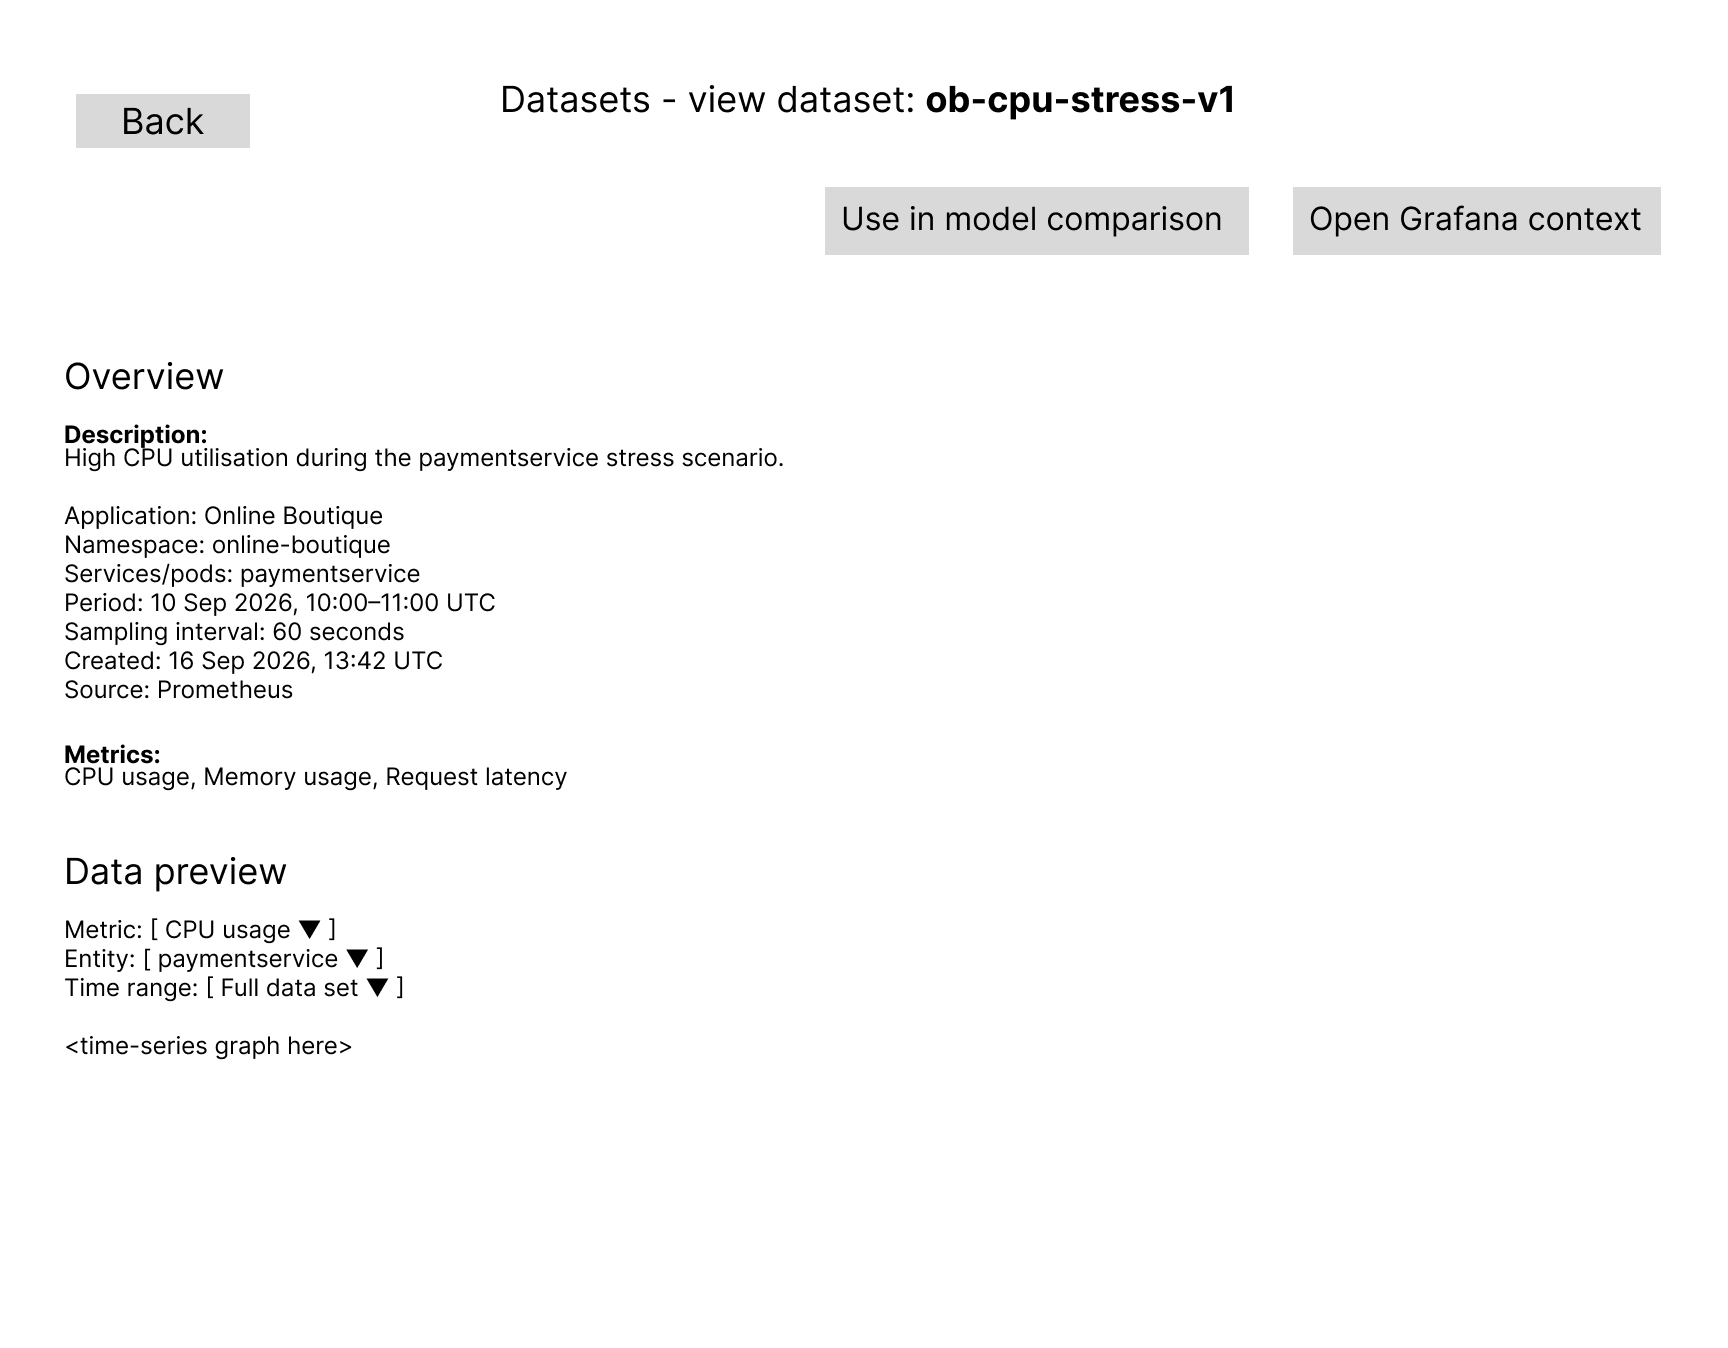
\includegraphics[width=1\linewidth]{figures/design/data_catalogue/Data Catalogue - view dataset.png}
    \caption{Data Catalogue: View Dataset}
    \label{fig:data_cat_view_dataset}
\end{figure}

\subsection{Managing Model Detectors and Training Pipeline}
In its current form, CloudSentinel is limited to the CGNN anomaly detection algorithm. However, under realistic circumstances, a framework like CloudSentinels would provide operators to have access to an algorithm of their own choosing rather than be forced to resort a single hardcoded detection algorithm. As such, the revised version of CloudSentinel is designed to incorporate functionality for adding custom detection algorithms. To incorporate this functionality, a custom adapter interface will be developed that operators can use to attach their own algorithm-implementations to. Ideally, an operator could develop and then 'drop' his algorithm implementation in a folder, where it will be discovered by CloudSentinel for later use.

The figures below display a low-fi design of the user interface layout. Figure \ref{fig:trained_models_overview} provides an entry point for inspecting the detector models available in the framework. Rather than treating a trained model as an isolated file, the design presents it as a managed artefact with identifiable metadata and a clear relationship to the detector implementation from which it was produced. The intent is to support data provenance in that operators are able to determine which model is available for use and subsequently inspect the configuration and training data associated with it.\\

Figure \ref{fig:register_detector_model} displays the workflow for registering an anomaly-detection algorithm. The interface is intended to make detector implementations discoverable and selectable without requiring changes to other parts of CloudSentinel. A registered detector can later be used in the training and comparison workflows. This design addresses the limitation of the baseline framework, which was restricted to a single hard-coded CGNN detector and did not demonstrate a clear mechanism for replacing or extending analytics components.\\

Figure \ref{fig:view_detector_details} displays the detector-details view, which provides the information required to understand the capabilities and requirements of a registered detector before it is used. More specifically: it gives operators a place to inspect the detector’s identity, implementation details, and supported configuration options. Some important information it provides are the data modality of the model (i.e. whether it supports metrics, logs or traces) as well as the  format of the expected input data, which as a default is expected to be Multivariate time series data. Generally, different anomaly-detection approaches may have different input requirements, parameters, and output semantics. The view therefore also helps separate detector-specific concerns from the broader dataset-management and training workflow.\\

Figure \ref{fig:train_new_models} displays the model-training screen. The model-training screen guides the operator through the selection of a detector and a previously stored dataset configuration. This replaces the earlier process in which training arrays had to be manually prepared, uploaded, and associated with a model through several disconnected steps. The design deliberately connects model training to the data catalogue so that the selected training data can be recorded as part of the resulting model artefact. In this way, the workflow makes the relationship between a trained model, its input data, and its detector implementation explicit.\\

Figure \ref{fig:train_review_screen} displays the review screen, which is the last step before starting training. It summarises the selected detector, dataset, and relevant configuration choices. Its purpose is to give the operator an opportunity to verify the training setup and reduce the risk of creating a model with unintended inputs or settings. Once training is started, these choices should be retained as model provenance metadata. This supports reproducibility by allowing a later user to determine which data and configuration were used to produce a particular model, rather than relying on undocumented interface state or manual record keeping.\\

% DETECTORS & TRAINING
\begin{figure}[H]
    \centering
    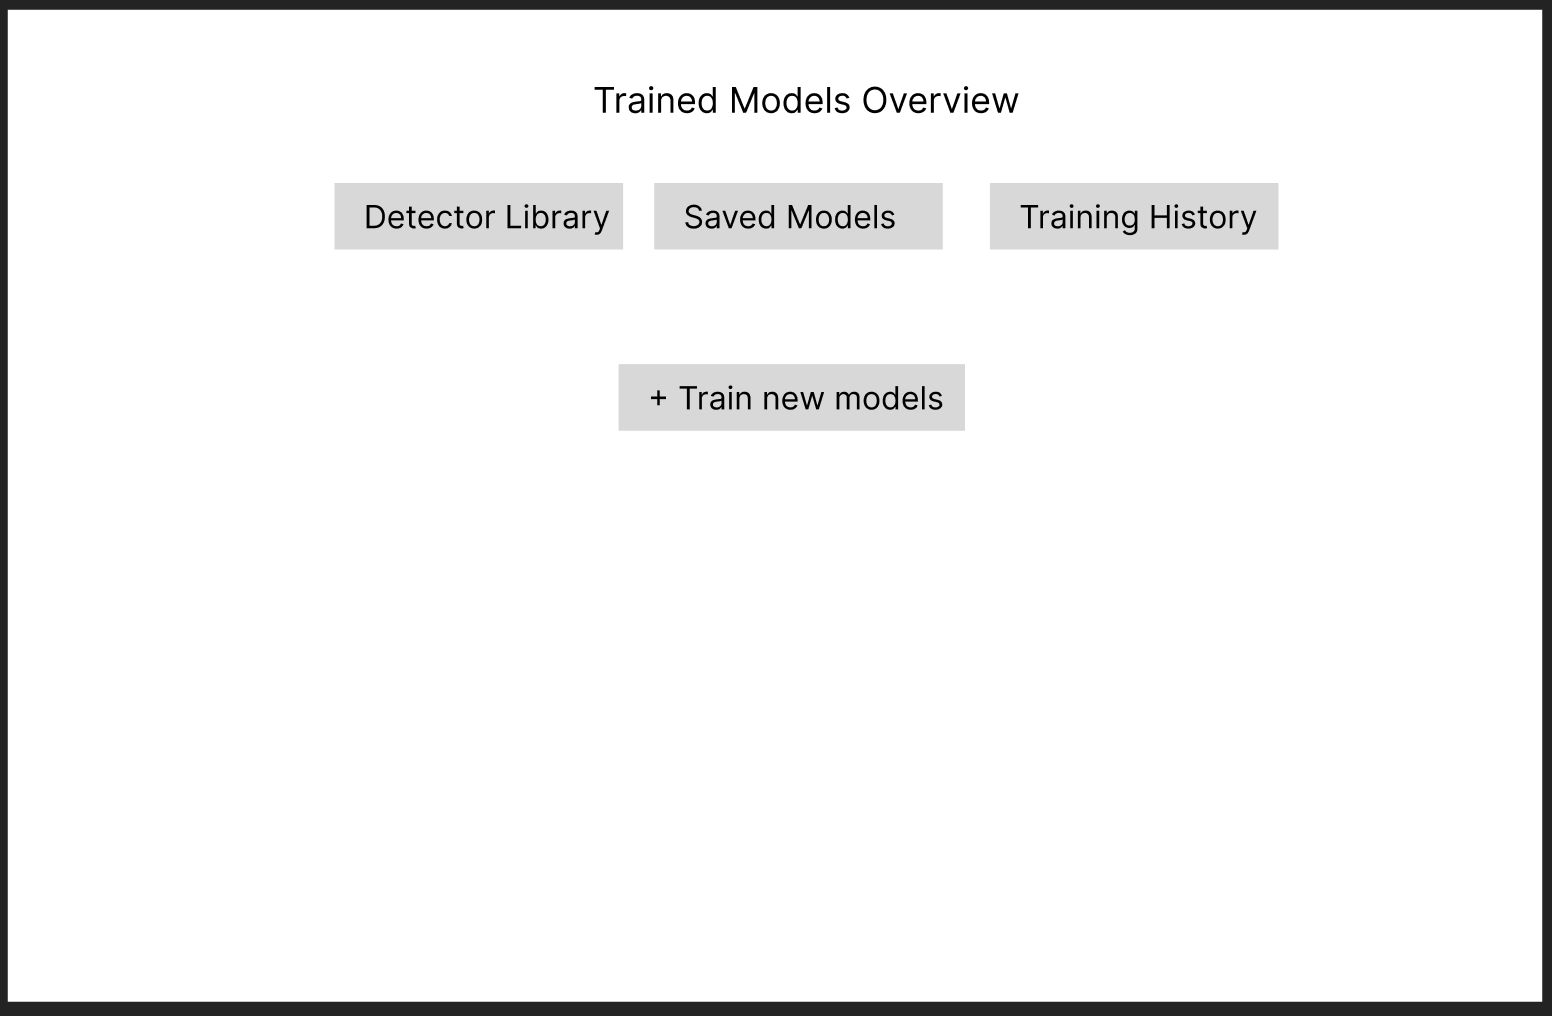
\includegraphics[width=1\linewidth]{figures/design/Training_and_importing/Screenshot 2026-09-24 at 01.17.15.png}
    \caption{Trained Models overview}
    \label{fig:trained_models_overview}
\end{figure}

\begin{figure}[H]
    \centering
    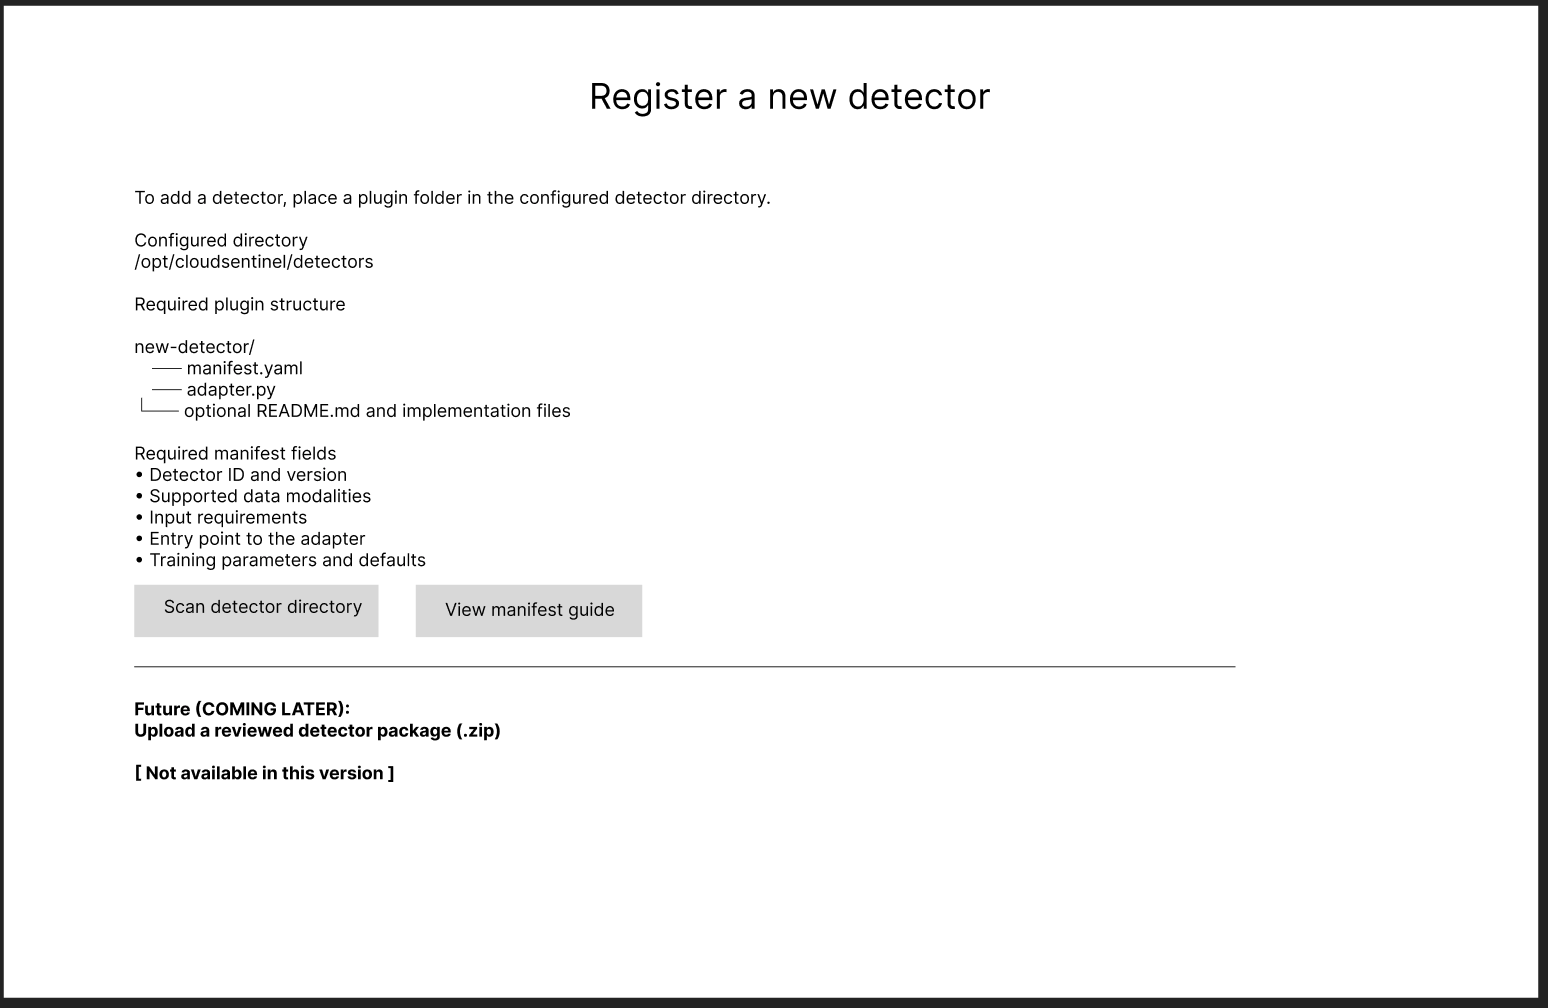
\includegraphics[width=1\linewidth]{figures/design/Training_and_importing/Screenshot 2026-09-24 at 01.17.23.png}
    \caption{Register a new detector}
    \label{fig:register_detector_model}
\end{figure}

\begin{figure}[H]
    \centering
    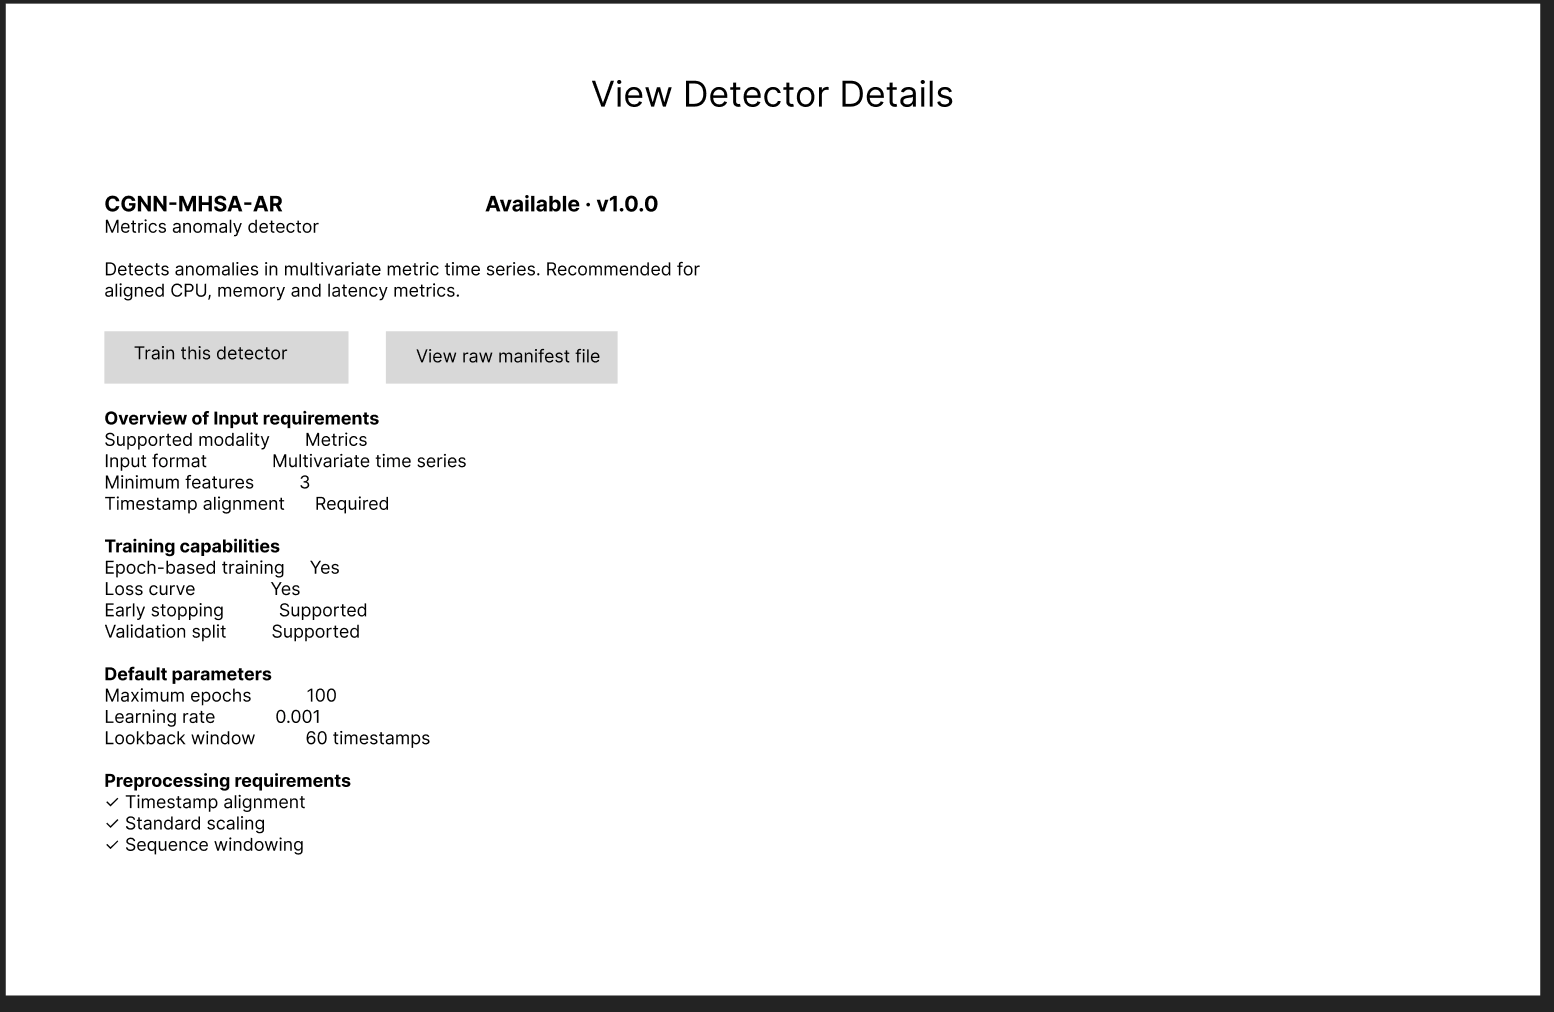
\includegraphics[width=1\linewidth]{figures/design/Training_and_importing/Screenshot 2026-09-24 at 01.17.34.png}
    \caption{View Detector Details}
    \label{fig:view_detector_details}
\end{figure}

\begin{figure}[H]
    \centering
    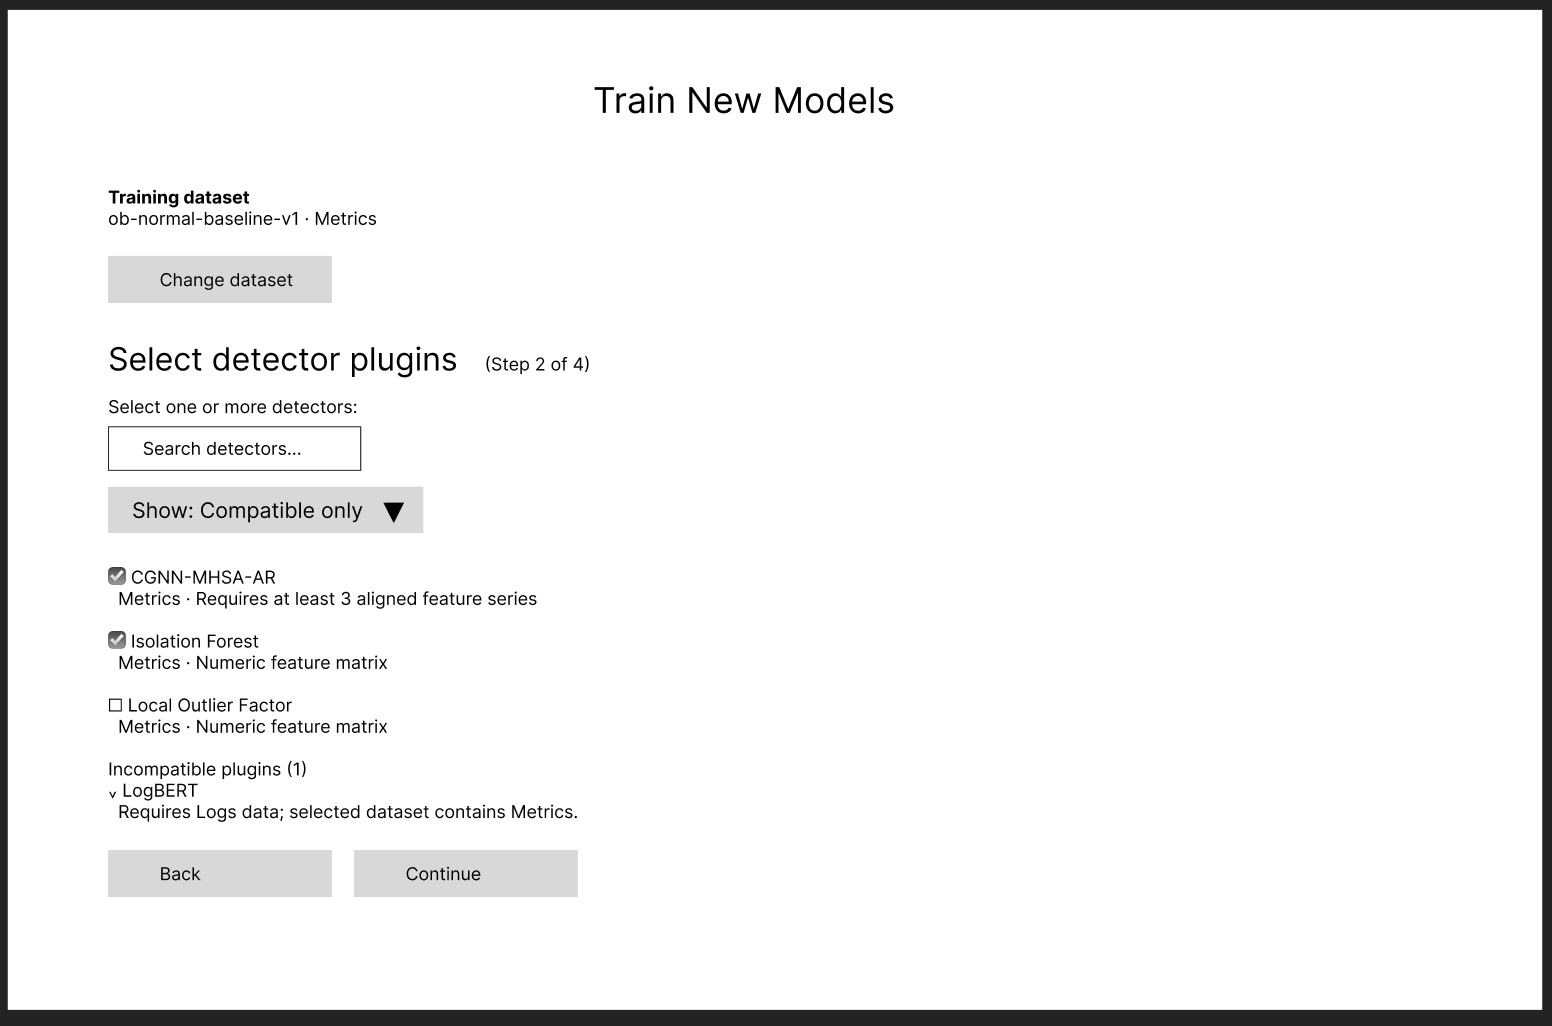
\includegraphics[width=1\linewidth]{figures/design/Training_and_importing/Screenshot 2026-09-24 at 01.17.53.png}
    \caption{Train New Models}
    \label{fig:train_new_models}
\end{figure}

% TRAINING MODELS USING THE DETECTORS
\begin{figure}[H]
    \centering
    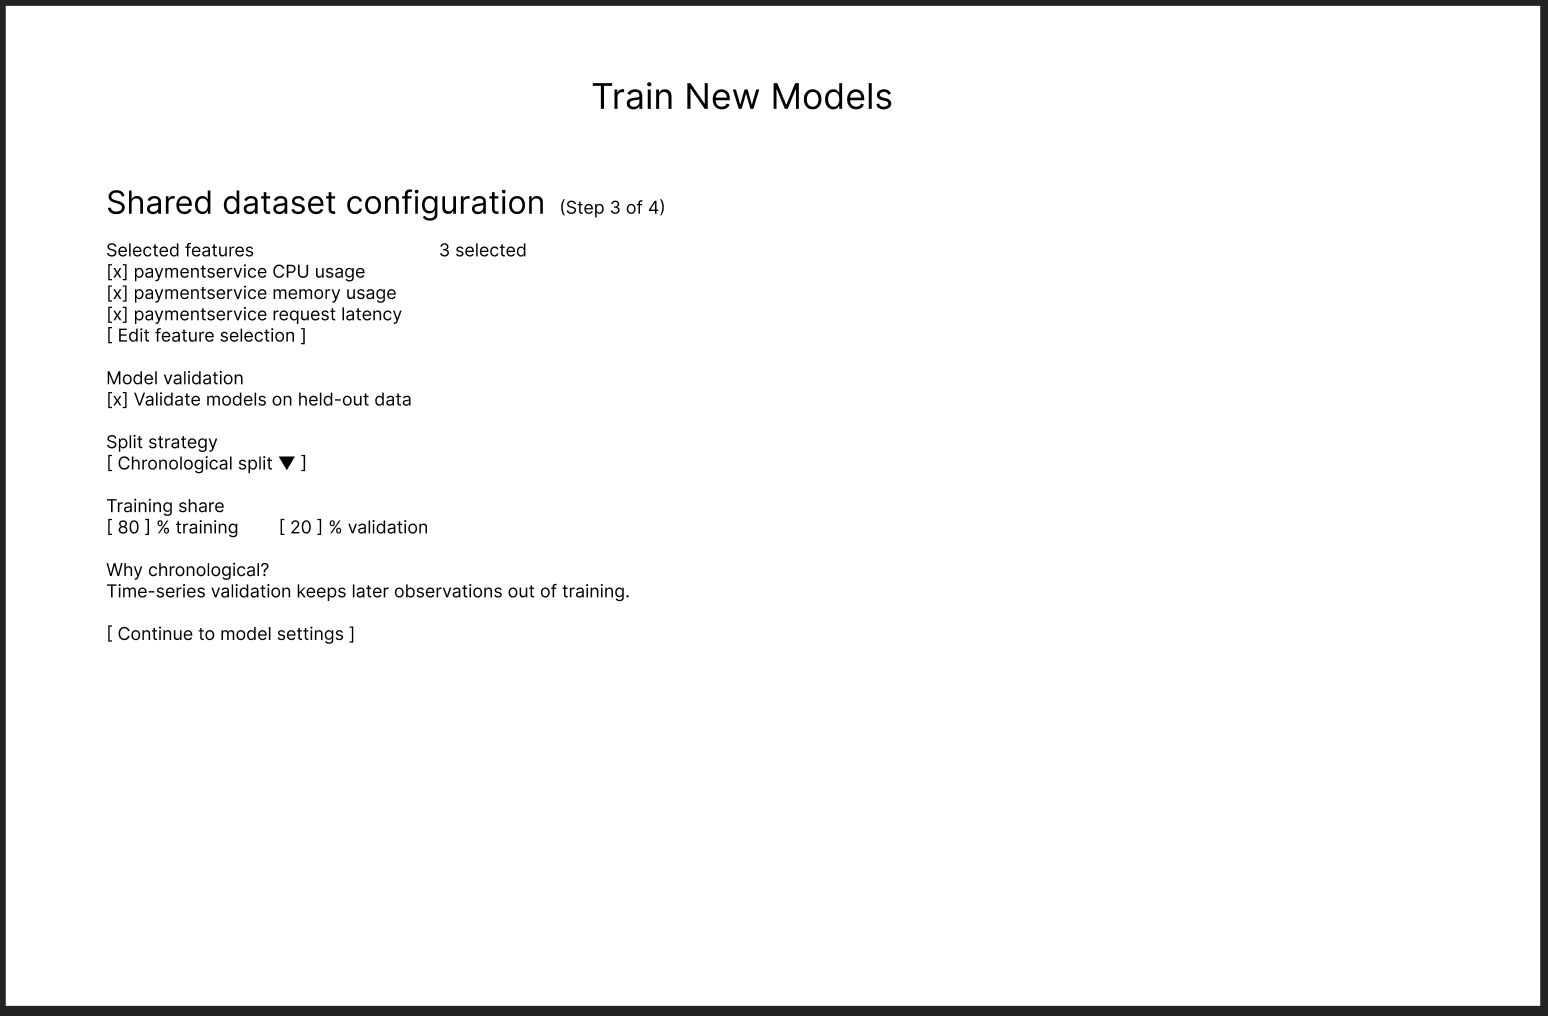
\includegraphics[width=1\linewidth]{figures/design/Training_and_importing/Screenshot 2026-09-24 at 01.18.01.png}
    \caption{Train New Models: Review Screen}
    \label{fig:train_review_screen}
\end{figure}

\subsection{Model Comparisons}
In order to make an assessment of what model to use, as well as being able to compare detector algorithms with each other, we introduce a Model Comparison component, which allows users to select a dataset with a given workload context (e.g. CPU usage spike anomaly), and run each model against the dataset, producing insightful evaluation metrics in the process that let operators compare their trained models. In order for the operator to be able to make an insightful assessment, three criteria points are applied. The first criterion is \textit{accuracy}, which is expressed as F1, precision and recall. The second criterion is \textit{lead time}, which is the time by which a model is able to predict an anomaly from occurring beforehand. The third criterion is \textit{robustness}, which we define as the degree to which a model is able to deliver consistent anomaly detection results across different workload contexts (for instance: low vs high activity datasets).\\

Figure \ref{fig:comparison_overview_screen} displays the comparison overview screen, which provides operators with a central location for managing previously executed anomaly-detection model comparisons. Rather than evaluating models in isolation, the design treats each comparison as a persistent evaluation artefact that records the evaluated models, the dataset used, and the resulting performance measures. This allows operators to revisit earlier evaluations, inspect their outcomes, and distinguish completed comparisons from those that still require execution or review.

Figure \ref{fig:comparison_new_comparison_screen} displays the 'new comparison' screen, which is essentially a guided workflow for the user for creating a new anomaly-detection comparison. The operator first selects a saved evaluation dataset and then chooses one or more trained model artefacts to evaluate on that same data. Requiring a shared evaluation dataset is important because it ensures that differences in the results can be attributed to the models and their configurations rather than to differences in input data. The review step makes the selected dataset, models, incident context, and intended evaluation measures visible before execution. This helps prevent accidental comparisons of incompatible artefacts and supports a more reproducible evaluation workflow.

Finally, figure \ref{fig:comparison_results_screen} displays the comparison results screen. This view brings together the information required to interpret model behaviour in one place. It presents a summary of the compared models and their evaluation measures, including precision, recall, F1-score, and lead time, while also retaining the associated training dataset and detection threshold for each model. The timeline view links model scores and thresholds to the known anomaly interval, enabling operators to inspect not only aggregate performance but also when each model identified anomalous behaviour. In addition, the detailed model view and provenance links allow the user to trace an observed result back to the model and training data that produced it. The design therefore supports a more informed model-selection process than relying on a single score or an untraceable trained artefact.

\begin{figure}[H]
    \centering
    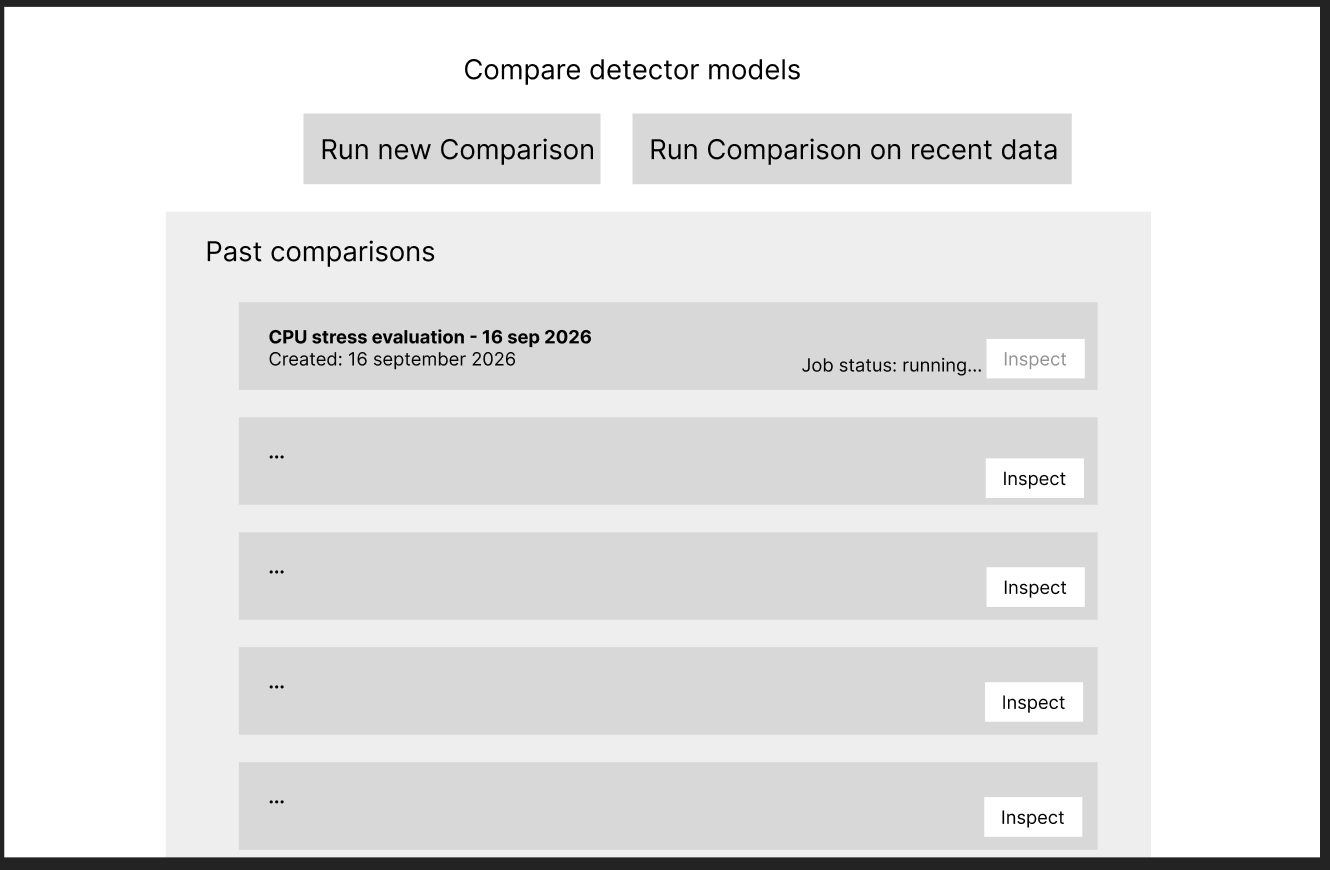
\includegraphics[width=1\linewidth]{figures/design/model_comparisons/Screenshot 2026-09-24 at 00.41.24.png}
    \caption{Compare Detector Models: Overview screen}
    \label{fig:comparison_overview_screen}
\end{figure}

\begin{figure}[H]
    \centering
    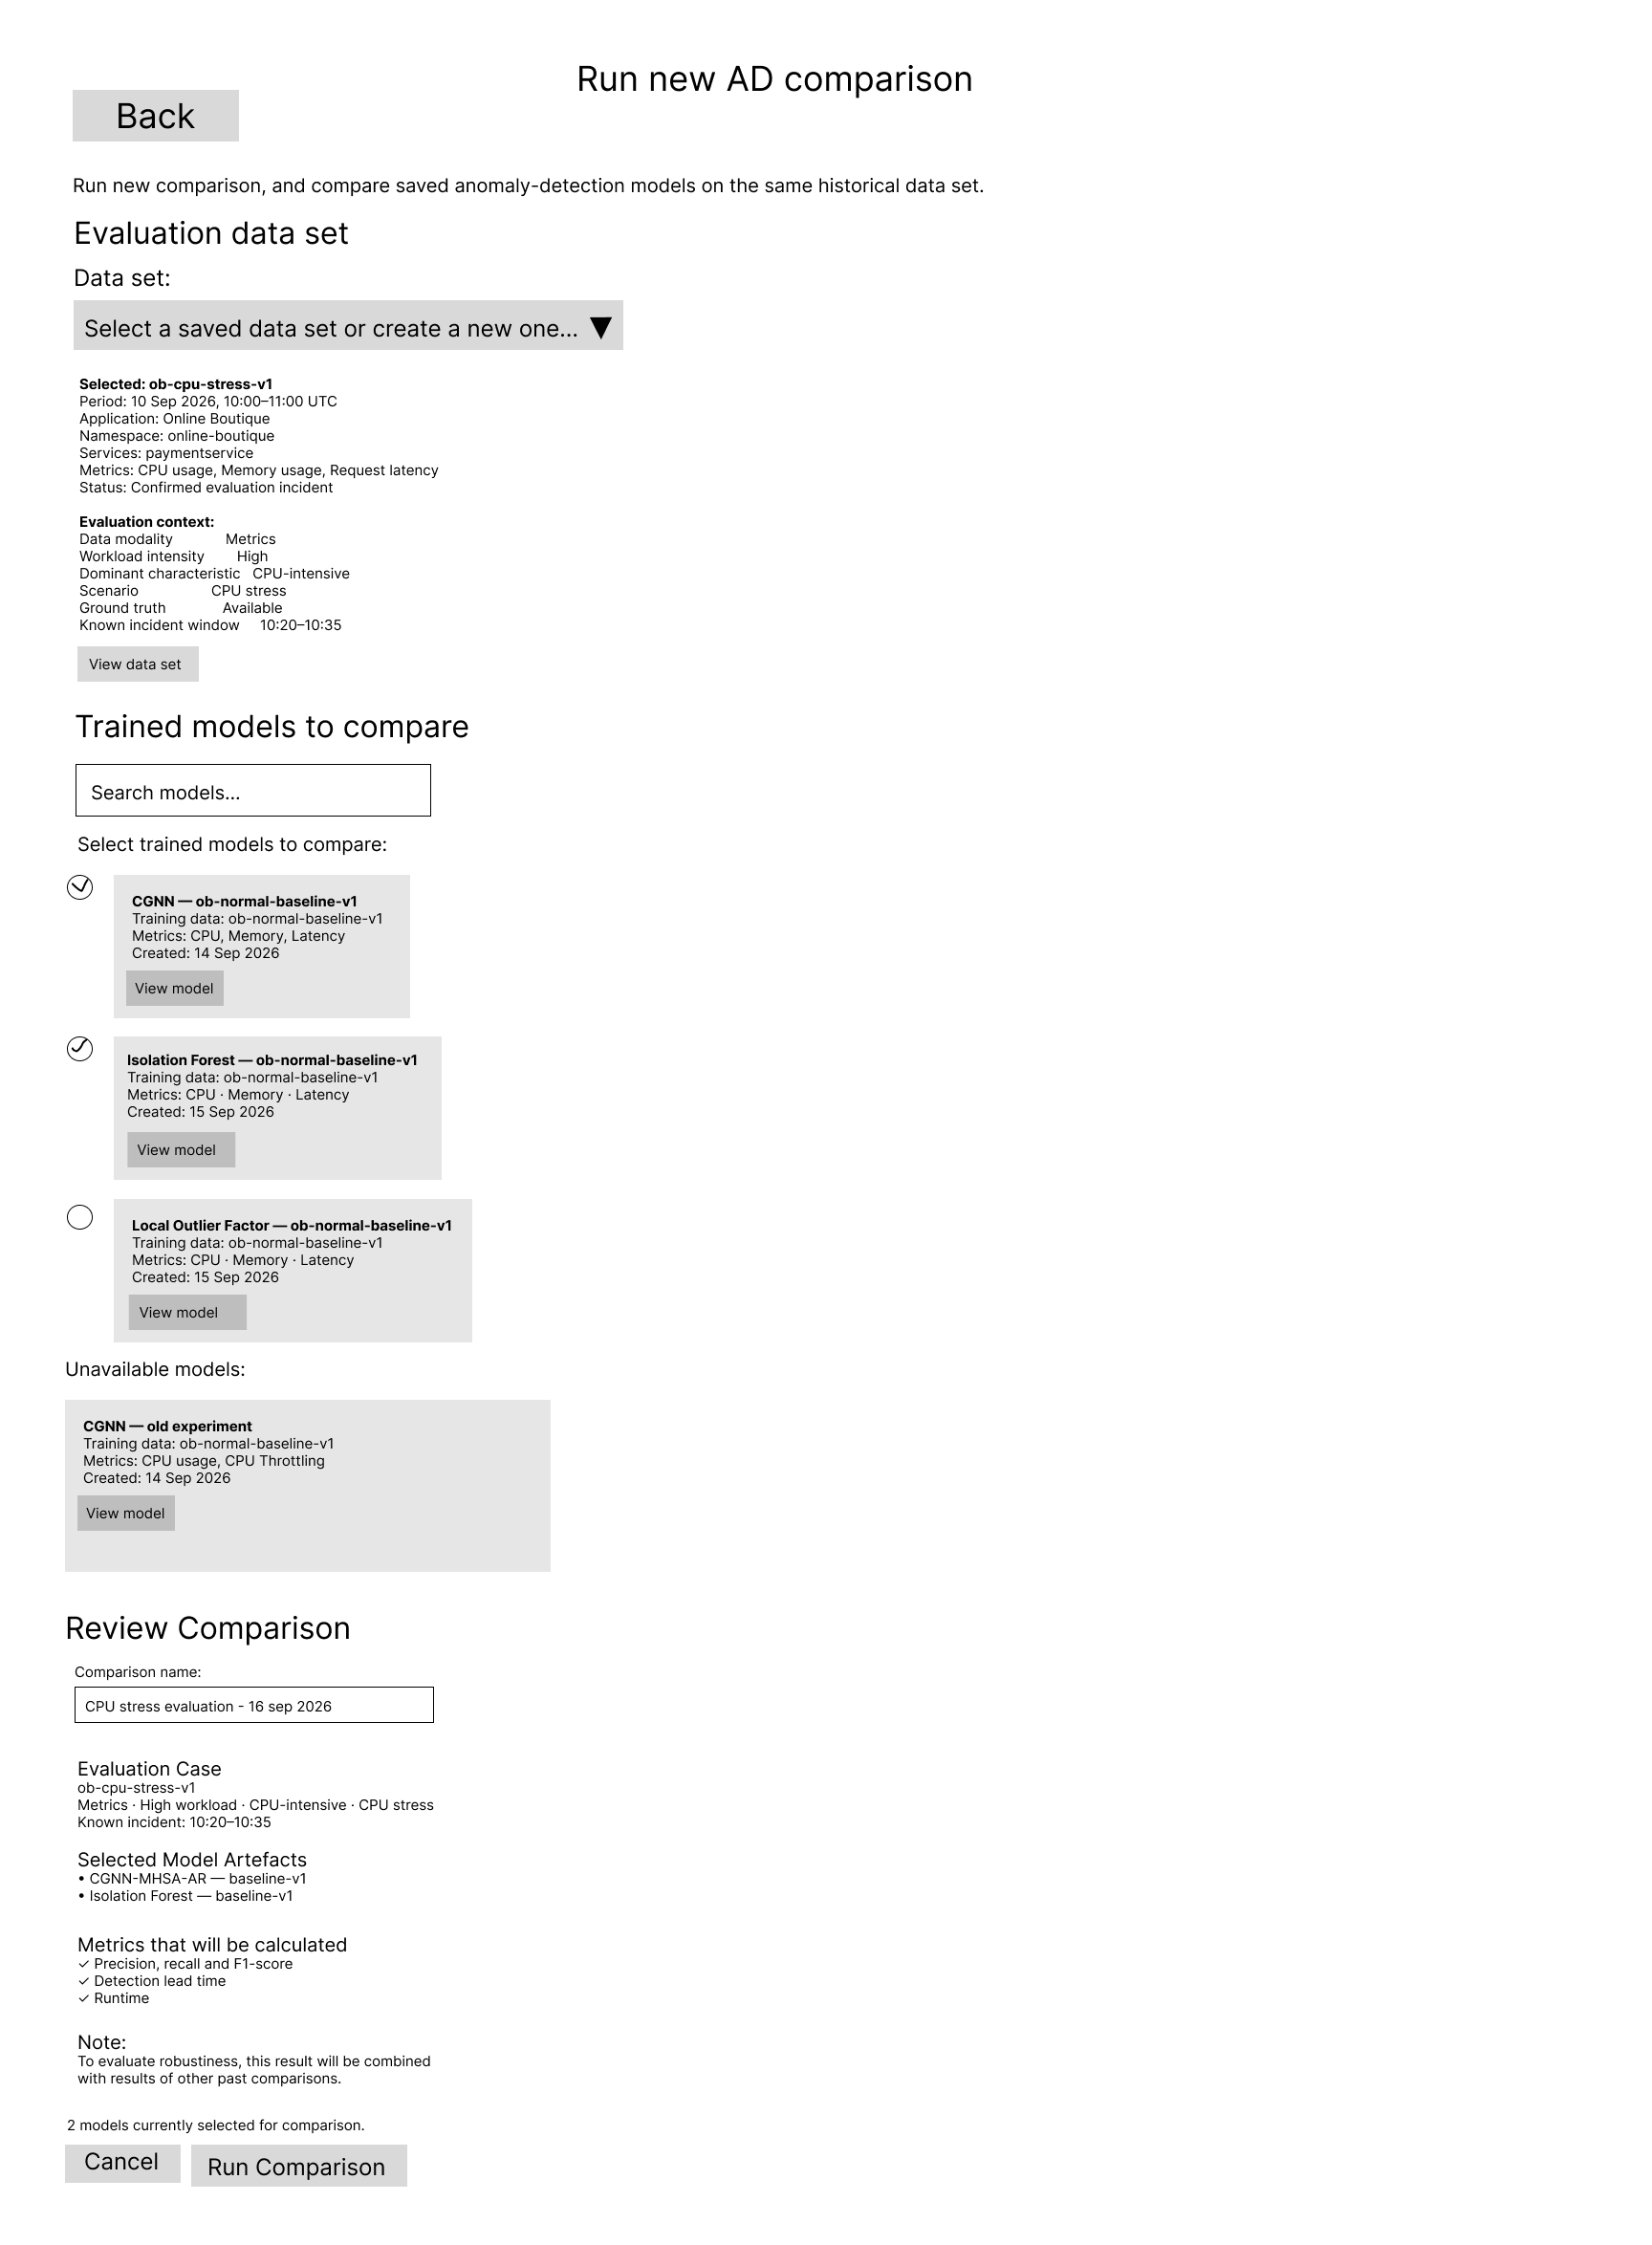
\includegraphics[width=1\linewidth]{figures/design/model_comparisons/Compare AD models - run new comparison.png}
    \caption{'Run new comparison' screen}
    \label{fig:comparison_new_comparison_screen}
\end{figure}

\begin{figure}[H]
    \centering
    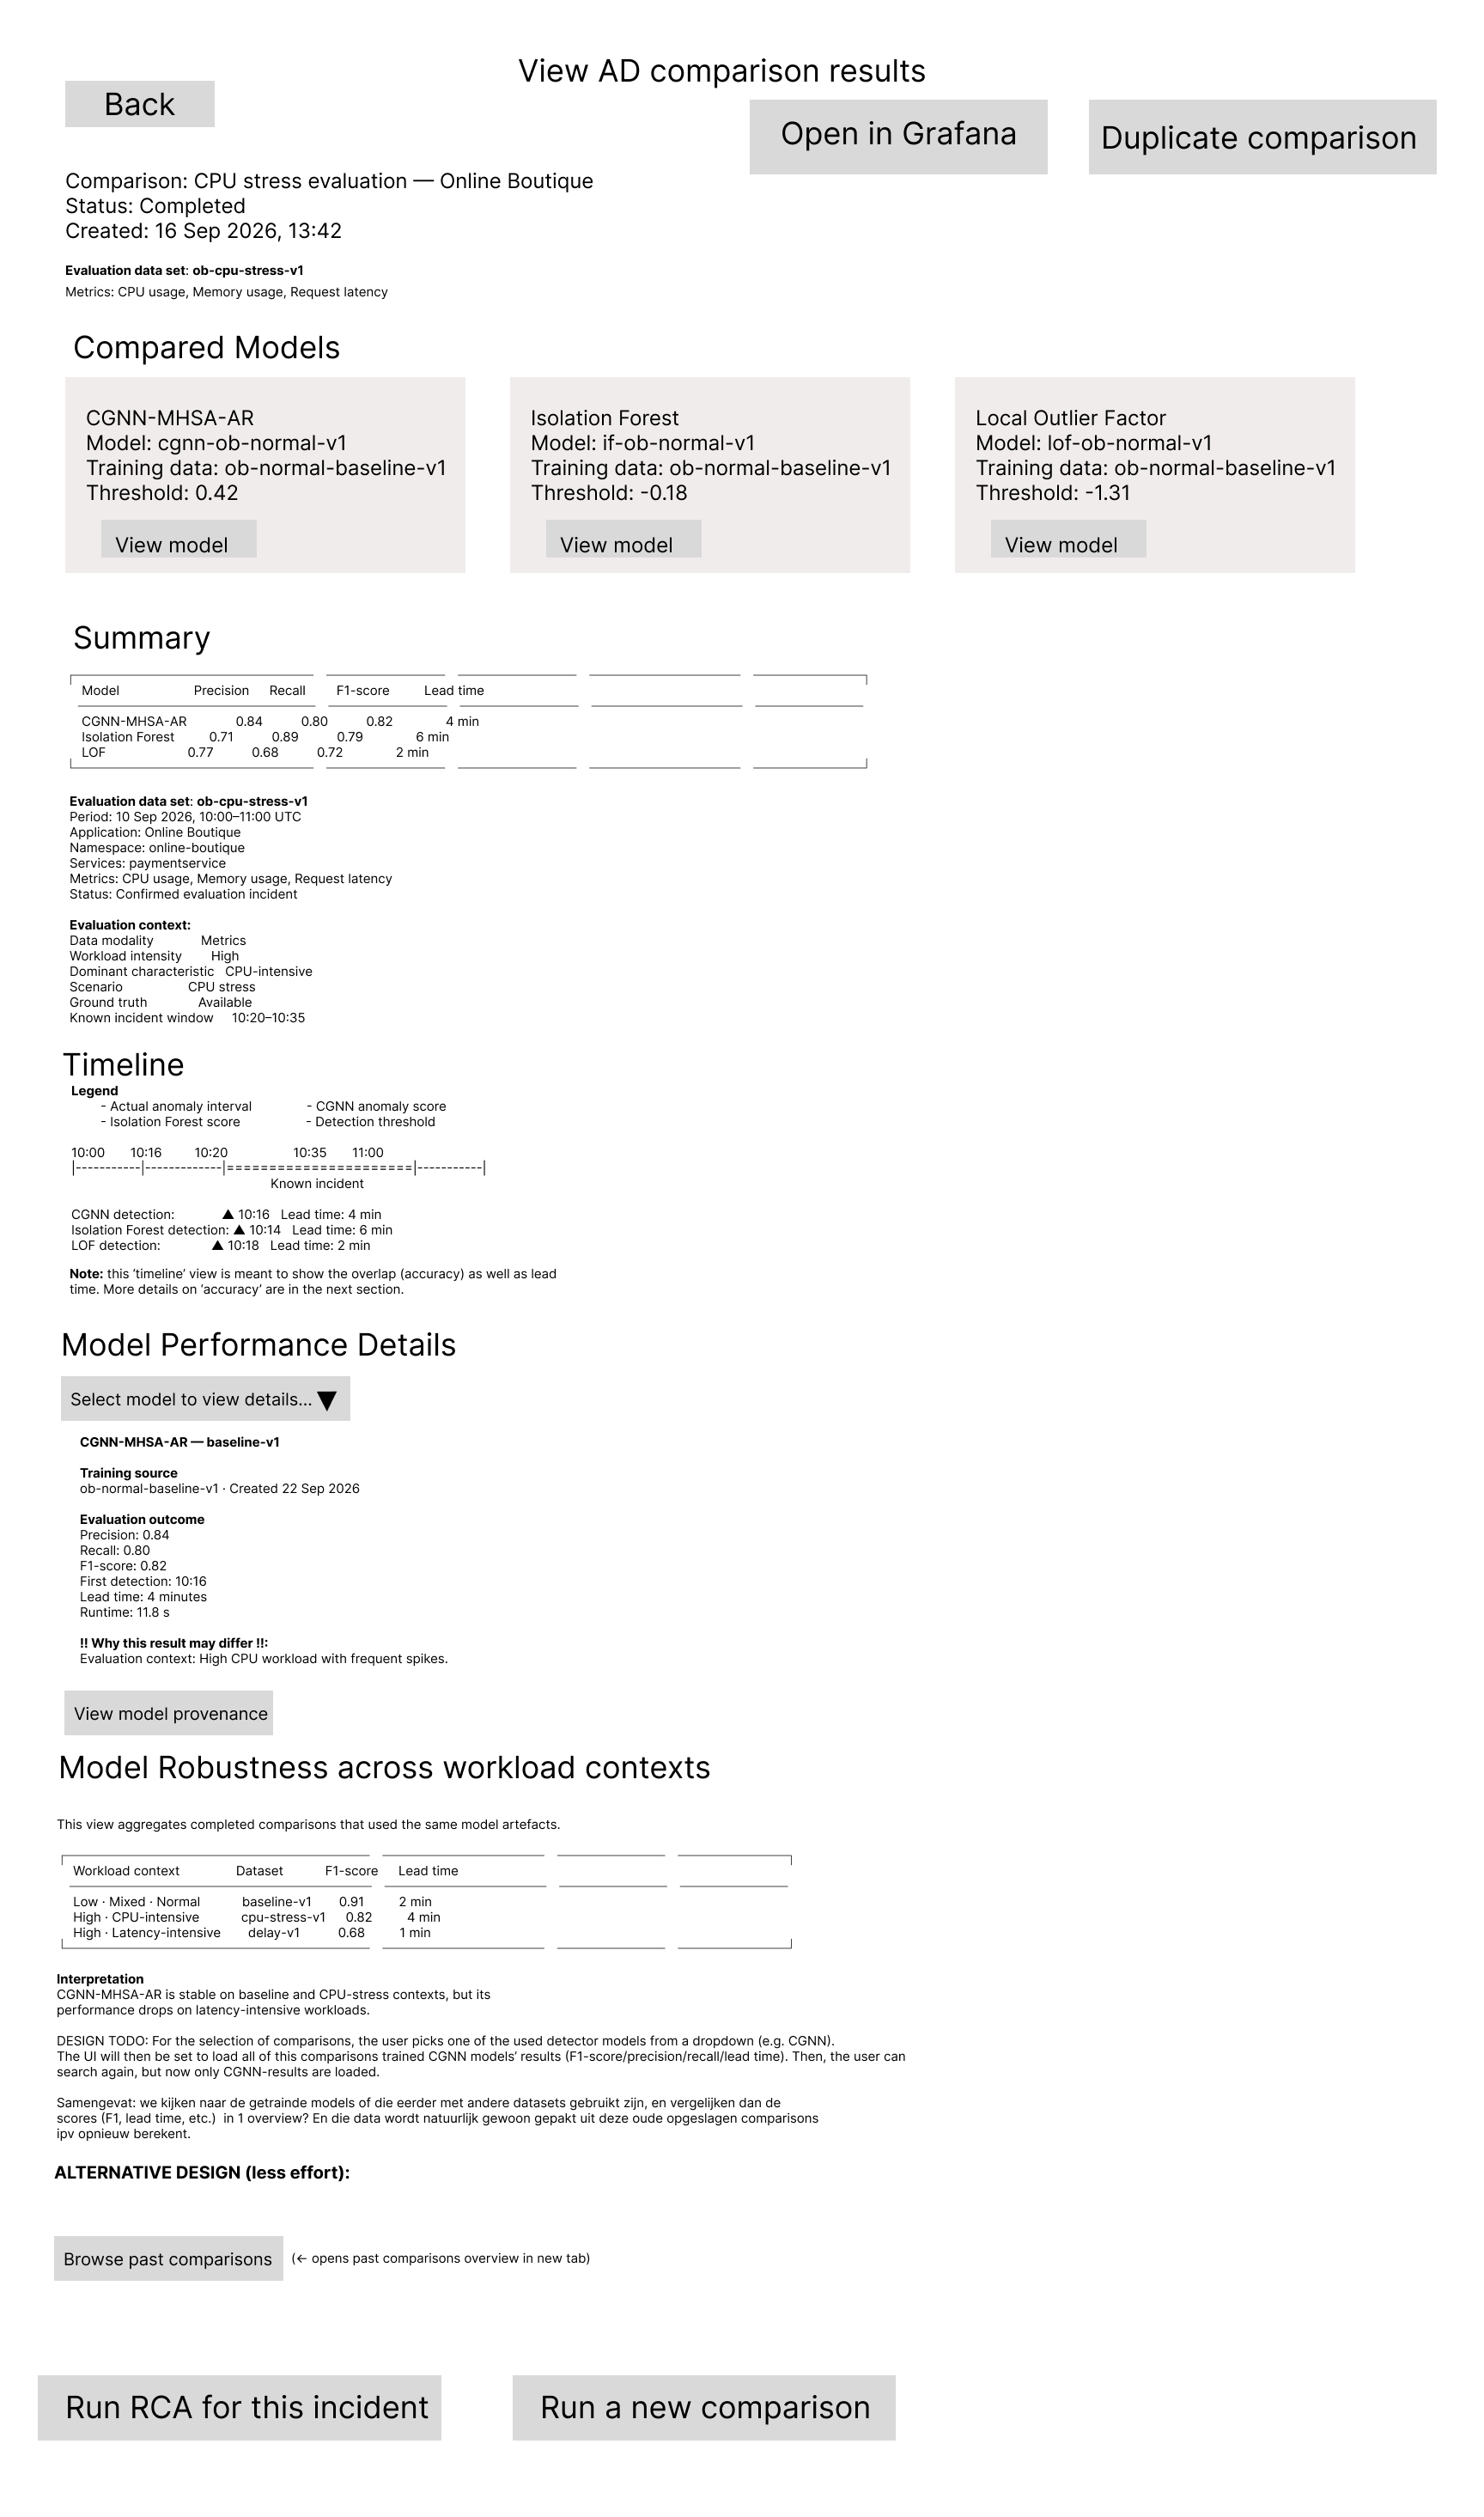
\includegraphics[width=1\linewidth]{figures/design/model_comparisons/comparison results.png}
    \caption{Comparison Results}
    \label{fig:comparison_results_screen}
\end{figure}

\subsection{Revised Live Monitoring}

The existing live-monitoring workflow also needs to be revised so that it continues to work with the other proposed changes. In the baseline framework, live monitoring is closely connected to the CGNN implementation and its own data-preparation and detection routes. This no longer fits a framework in which several detector plugins can produce Saved Models with different preprocessing and artefact formats.

The revised design therefore starts monitoring from one explicit Saved Model rather than from a general detector type. The monitoring pipeline should collect live Prometheus observations in the same feature order and with the same source configuration as the data used to prepare that model. It should then send these observations to the generic inference interface provided by the model's detector adapter. In this way, live monitoring can use CGNN, Isolation Forest, Local Outlier Factor, or a later compatible detector without adding a separate monitoring route for each one.

The monitoring interface should also retain the identity of the selected model and present the resulting anomaly information as a named session. Where the selected input and available monitoring evidence are suitable, an operator should be able to enable root-cause analysis for that session. The detailed monitoring-history and selectable RCA functions described later were not fully specified in the initial design. They were added during implementation after it became clear that short-lived task results were insufficient for revisiting and explaining live detections.

